\documentclass{article}
\usepackage{tikz}
\usetikzlibrary{arrows.meta}

\title{Unicidad Digrafo}
\author{Josefina Negrotto, redaccion: Daniel Bustos}
\date{27 de abril de 2024}

\begin{document}
\maketitle

Sea $G = (E,V)$ un grafo orientado, con cada vértice un grado distinto de salida. Formalmente:
\[
\forall v \in V, w \in V, v \neq w \Rightarrow d_{\text{out}}(v) \neq d_{\text{out}}(w)
\]

Podemos ordenarlos por orden creciente:
\[
d_{\text{out}}(v_1) < d_{\text{out}}(v_2) < \ldots < d_{\text{out}}(v_n)
\]

\textbf{Observación:} Como el grado máximo de salida es $n - 1$ y el mínimo 0, como todos deben ser distintos, vale que $d_{\text{out}}(v_i) = i - 1$.

Observemos que para el vértice $v_n$ debe tener grado de entrada 0, ya que está relacionado con todos los demás, y (por ser grafo orientado) si existe la relación $v_n \to v_i$ no existe la relación $v_i \to v_n$. Entonces $d_{\text{in}}(v_n) = 0$. Análogamente $d_{\text{in}}(v_{n-1}) = 1$, ya que solo puede recibir del grafo $v_n$.

Fácilmente se ve que el grado de $d_{\text{in}}(v_i) = n - i$. (Podemos probarlo por inducción)

Luego para todo vértice $v \in V$ vale que $d_{\text{in}}(v_i) + d_{\text{out}}(v_i) = n - i + i - 1 = n - 1$. Entonces viendo el grafo subyacente (el grafo direccionado convertido a grafo normal) Todos los vértices son universales. Luego el único grafo con $n$ nodos que cumple lo pedido es el grafo completo, dándonos la unicidad.

\begin{figure}[h]
\centering
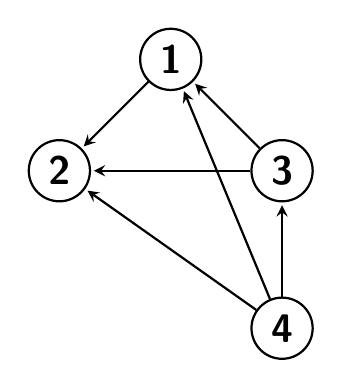
\begin{tikzpicture}[
    > = stealth, % arrow head style
    shorten > = 1pt, % don't touch arrow head to node
    auto,
    node distance = 2cm, % distance between nodes
    thick, % line style
    main node/.style={circle,draw,font=\sffamily\Large\bfseries}
  ]
  
  % Nodes
  \node[main node] (1) {1};
  \node[main node] (2) [below left of=1] {2};
  \node[main node] (3) [below right of=1] {3};
  \node[main node] (4) [below of=3] {4};

  % Edges
  \path[every node/.style={font=\sffamily\small}]
    (1) edge[->] node {} (2)
    (3) edge[->] node {} (1)
    (3) edge[->] node {} (2)
    (4) edge[->] node {} (1)
    (4) edge[->] node {} (2)
    (4) edge[->] node {} (3);
\end{tikzpicture}
\caption{Digrafo: (1,2)(3,1)(3,2)(4,1)(4,2)(4,3) .\\ 
        Es facil ver que el grafo adyacente es completo}
\end{figure}

\end{document}
